
%(BEGIN_QUESTION)
% Copyright 2012, Tony R. Kuphaldt, released under the Creative Commons Attribution License (v 1.0)
% This means you may do almost anything with this work of mine, so long as you give me proper credit

The following schematic diagram shows a Westinghouse model CO-11 overcurrent protective relay, complete with time-overcurrent (``CO''), instantaneous overcurrent (``IIT''), and seal-in (``ICS'') elements.  The relay as shown has been removed from service, and is sitting on a workbench ready to be tested by a technician:

$$\includegraphics[width=15.5cm]{i01172x01.eps}$$

Sketch all necessary connecting wires to allow testing of {\it only} the time-overcurrent (51) function.  An adjustable AC current source provides input power to the relay, while a light bulb serves to indicate when the relay's trip contact(s) have closed.

\underbar{file i01172}
%(END_QUESTION)





%(BEGIN_ANSWER)

{\it Grading is all-or-nothing.  Either the circuit is connected properly, or it is not.}  

$$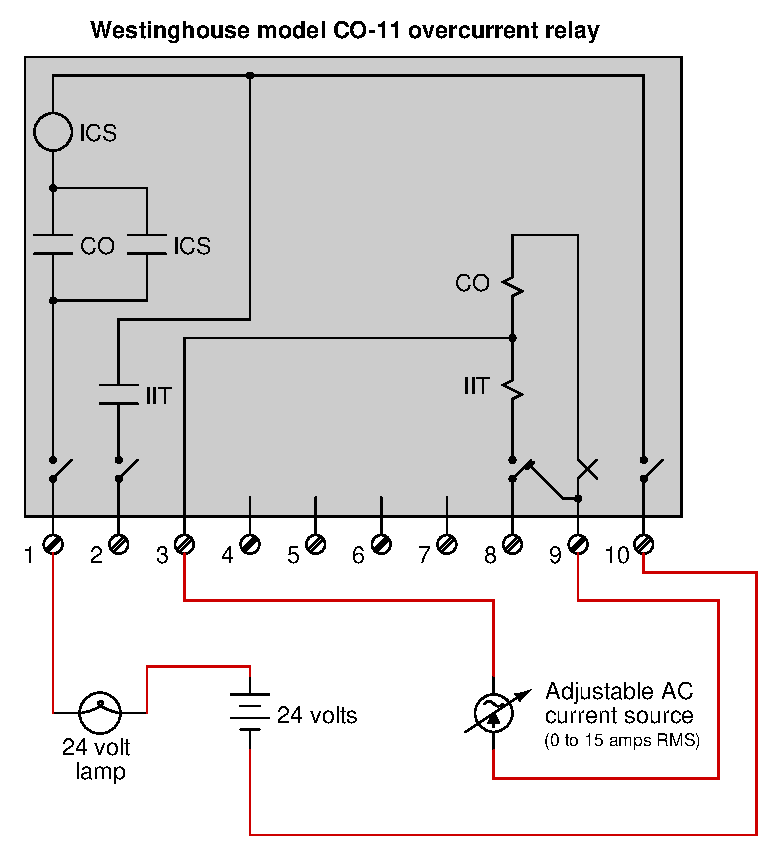
\includegraphics[width=15.5cm]{i01172x02.eps}$$

Note: it is also permissible to connect the adjustable AC current source to terminals 8 and 9, rather than 3 and 9.  This will have the effect of energizing both the CO and IIT coils, but the CO function will still be tested adequately.  Polarity is irrelevant, both for the AC test current source as well as the 24 VDC light bulb trip indicator circuit.
 
%(END_ANSWER)





%(BEGIN_NOTES)

{\bf This question is intended for exams only and not worksheets!}

%(END_NOTES)


